\newpage
\subsubsection{Two Square \& Multiply algorithms and the factor method}

\begin{itemize}
\item  	\begin{tabularx}{\linewidth}{ p{16cm} p{1.5cm}}
		LtoR Square \& Multiply - 
		\textit{Chandah-sutra of Pingala, a classic Hindu, 400AC}-  & $0\%$ \\ 
		\end{tabularx}	
			\noindent
			Method designed following the observation that squaring can faster than multiplying.
			A square is done each time that is scanned another bit of the exponent.
			A multiplication is done conditionally depending on the value ofthe scanned bit.
						
			Since $n > 4$ this is computationally more efficient than naive exponentiation.
			This method uses the same addition chain that 'Multiply always' but the same one than the LtoR Binary method.\\	
			\begin{figure}[h]
				\begin{center}
				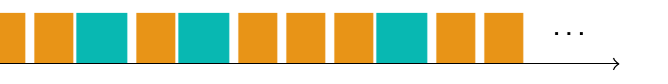
\includegraphics[scale=0.33]{images/SM.png}		
				\caption{$d_2 = 0 1 1 0 0 1 0 0 ... $}
				\end{center}
			\end{figure}	
			\begin{algorithm}[h]
				\KwIn{$x, {d =  d_{t-1} ... d_1 d_0}_{2}$}
				\KwOut{ $ y   =  x^d \mod n$ }
				 $y \leftarrow 1$ \;
				\For{$i  \gets t-1$ \textbf{to} $0$}
				{
				$y \leftarrow y^2 \mod n$\\				 
				\If{ $d_i= 1$  }{ 
					$y \leftarrow y \times x \mod n$	 
					} 
				}									 
				\Return{$ y $}\;
				\caption{LtoR dichotomic exponentiation}
			\end{algorithm}	

			\underline{Example :} LtoR Square \& Multiply: $n=23_{10}=10111_2$ the method starts 
			from the MSB.
			
			\begin{tabularx}{\linewidth}{ p{2cm} p{12cm} p{2cm}}
				$y=1$ & $ $\\
				$y:=y^2$ & $y:=y*x$	& $(y=x)$\\		
				$y:=y^2$ &       	& $(y=x^2)$\\
				$y:=y^2$ & $y:=y*x$ & $(y=x^{5})$\\
				$y:=y^2$ & $y:=y*x$ & $(y=x^{11})$\\
				$y:=y^2$ & $y:=y*x$ & $(y=x^{23})$
			\end{tabularx}	
			Powers of $x$ successively computed:	
			$x$ $x^2$ $x^4$ $x^5$ $x^{10}$ $x^{11}$ $x^{22}$ $x^{23}$, length 8\\
			
			\textit{Names}\\
			Algorithm also known as: 
			dichotomical exponentiation, Square \& Multiply, binary method. \\
			Do not mistaken this algorithm with its atomic version  as it is not 
			using a specialized routine for squaring it is also called sometime 
			'Multiply always'...		
							
			Note that the first non trivial step is always the same as we have 
			$d_{t_{min}-1} $, and will result in $y=x$ and therefore the it can be replaced for 
			an if.

			Which leads the number of operations to be performed to:
			\begin{center}
				$t_{min} + \omega_{\mathcal{H}}(d)-2$\\
				with $t_{min} =  \lfloor log_2(d) \rfloor$
			\end{center} 
			\newpage

\item  	\begin{tabularx}{\linewidth}{ p{16cm} p{1.5cm}} 
		RtoL Square \& Multiply-
		\textit{Al Kashi, 1427 AC}-  & $0\%$ \\
		\end{tabularx}	
			\noindent	

		Those two algorithms are exactly the same, those two versions are presented here.
		The fist version is scanning the bit form Right to Left, the second one is doing the 
		conversion on the fly starting from $d$.
		\textit{ $d_i= 1$ vs $d  \leftarrow \lfloor \frac{d}{2} \rfloor $ }.\\\\
		\begin{algorithm}[h]
			\KwIn{$x,n \in \mathbb{N}$, $x \leq n$}
			\KwOut{ $ y   =  x^d \mod n$ }
			$y \leftarrow 1$ \;		
			$local \leftarrow x$ \;	
			\While{$d  \neq 0$ }{			 
			    \If{ $d \mod 2 = 1$  }{ 
			    	$y \leftarrow y \times local \mod n$	\;
				} 
			$d  \leftarrow \lfloor \frac{d}{2} \rfloor $\;
			$local \leftarrow y^2 \mod n$	
			}									 
			\Return{$ y $}\;
			\caption{RtoL dichotomic exponentiation -On the fly version-}
		\end{algorithm}		
		\begin{algorithm}[h]
			\KwIn{$x,n \in \mathbb{N}$, $x \leq n$, ${d =  d_{t-1} d_1 d_0}_2$}
			\KwOut{$ y =  x^d \mod n$}
			$y \leftarrow 1$ \;		
			$local \leftarrow x$ \;	
			\For{$i \gets 0$ \textbf{to} $t-1$}{			 
			\If{ $d_i= 1$  }{ 	
				$y \leftarrow y \times local \mod n$	
				} 
			$local \leftarrow y^2 \mod n$	
			}									 
			\Return{$ y $}\;
			\caption{RtoL dichotomic exponentiation}
		\end{algorithm}				

		\underline{Example:} RtoL Binary method: $n=15_{10}=1111_2$\\			
			\begin{tabularx}{\linewidth}{ p{2cm}  p{12cm} p{4cm}}
				$y=1  $ & $l=x$		& $(y=1,l=x)$\\
				$y:=y*l$ & $l:=l^2$ 	& $(y=x,l=x^2)$\\
				$y:=y*l$ & $l:=l^2$ 	& $(y=x^3,l=x^4)$\\
				$y:=y*l$ & $l:=l^2$ 	& $(y=x^7,l=x^8)$\\
				$y:=y*l$ &          	& $(y=x^{15},l=x^{16})$
			\end{tabularx}	
			Powers of $x$ successively computed:	
			$x$ $x^2$ $x^3$ $x^4$ $x^7$ $x^{8}$ $x^{15}$, length 7: 6 operations\\
			This is the smallest value of $n$ for which the binary method is not optimal:\\
			The factor method with $x^{15} = (x^{3})^{5}$, lead to 5 operations\\\\
		\underline{Example:} RtoL Binary method: $n=23_{10}=10111_2$\\			
			\begin{tabularx}{\linewidth}{ p{2cm}  p{12cm} p{4cm}}
				$y=1  $ & $l=x$		& $(y=1,l=x)$\\
				$y:=y*l$ & $l:=l^2$ 	& $(y=x,l=x^2)$\\
				$y:=y*l$ & $l:=l^2$ 	& $(y=x^3,l=x^4)$\\
				$y:=y*l$ & $l:=l^2$ 	& $(y=x^7,l=x^8)$\\
				         & $l:=l^2$  	& $(y=x^7,l=x^{16})$\\
				$y:=y*l$ &          	& $(y=x^{23},l=x^{16})$
			\end{tabularx}	
			Powers of $x$ successively computed:	
			$x$ $x^2$ $x^3$ $x^4$ $x^7$ $x^{8}$ $x^{16}$ $x^{23}$, length 8: 7 operations\\	

		Note that those algorithms are provided in a pedagogical way, in a real life implementation two multiplication can be skipped: the $d_i= 0$ step $y \leftarrow 1 \times x \mod n$ can be exchanged for a if. The last square is also useless and can be prevented.\\\\
		Which leads the number of operations to be performed to:
		\begin{center}
			$t_{min} + \omega_{\mathcal{H}}(d)-2$\\
			with $t_{min} =  \lfloor log_2(d) \rfloor$
		\end{center} 

\item  \begin{tabularx}{\linewidth}{ p{16cm} p{1.5cm}}
			Square \& Multiply Always  & $0\%$ \\ 
		\end{tabularx}	
		\label{Square_Multiply_Always}
		\noindent
		This a counter-measure, to prevent multiply vs non multiply discrimination.\\
		The SPA vulnerability of S$\&$M algorithms come from a possible square versus 
		multiply discrimination, coming from the algorithmic implementation of those routines.

			Solutions:
		\begin{itemize}
			\item \textit{'Mutliply Always' i.e. Naive 'Square \& Multiply'} \\
			replace squarings by multiplications, but slower still a condition remains ...
			\item \textit{'Square \& Multiply Always'} \\
			Whatever the need 'always multiply': if no multiplication is requirred place a bogus multiplication
			\begin{figure}[h]
				\begin{center}
	        	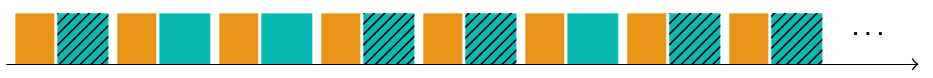
\includegraphics[scale=0.33]{images/SMA.png}
				\caption{LtoR Square \& Multiply Always illustration}
				\end{center}
			\end{figure}
			\item \textit{'Joye's Multiply Always' i.e. Atomic 'Square \& Multiply'} \\
			replace the squaring algorithm by a multiplying one: fully atomic algorithm.
		\end{itemize}

\item 	\begin{tabularx}{\linewidth}{ p{16cm} p{1.5cm}} 
		Square \& Multiply on the fly reduction-
		\textit{G.R.Blakley, 1983 AC}-  & $0\%$ \\
		\end{tabularx}	

\item 	Nota on Square \textit{vs} Multiply operands:

		When applying Square \& Multiply algorithm, additionally to the fact that
		the dedicated routines are different, there is structural difference between the two 
		fundamental operation:

		\begin{itemize}
			\item \textit{Square operations} possesses a variable operand, likely to change at each execution.
			\item \textit{Multiply operations} possesses a static operand, the $x$ to elevate to a certain power.\\
		\end{itemize}

\item 	\begin{tabularx}{\linewidth}{ p{16cm} p{1.5cm}} 
		Factor Method
		\textit{D.E.Knuth, 1908 AC}-  & $0\%$ \\
		\end{tabularx}	
		This method is recursive and is neither better or worst than the binary method.

		if $d$ is prime, compute $x \times x^{d-1}$\\
		if not and $d>3$, compute $ x^d = x^p \times x^{d'}$ with $p$ prime.

		The Factor Method is better than the binary method \textit{in average}.

		\underline{Example:} factor method: $n=15_{10}$\\			
			$x^{15} = (x^{3})^{5}$ and $x^{3} = x \times x^{2}$\\
			$x^{15} = x^{3} \times (x^{3})^{4}$\\
			$x^{15} = x^{3} \times ((x^{3})^{2})^2$\\
			Powers of $x$ successively computed:
			$x$ $x^2$ $x^3$ $x^6$ $x^{12}$ $x^{15}$, length 6: 5 operations\\
			This example is the first where the factor method is better than the binary method.

			But the factor method is not always better ...

		\underline{Example:} factor method: $n=33_{10} = 100001_2$\\			
			$x^{33} = (x^{3})^{11}$ and $x^{3} = x \times x^{2}$\\
			$x^{33} = x^{3} \times (x^{3})^{10}$\\
			$x^{33} = x^{3} \times ((x^{3})^{2})^5$\\	
			$x^{33} = x^{3} \times (x^{6})^5$\\
			$x^{33} = x^{3} \times x^{6} \times ((x^{6})^{2})^2$\\
			Powers of $x$ successively computed:
			$x$ $x^2$ $x^3$ $x^6$ $x^{12}$ $x^{24}$ $x^{30}$ $x^{33}$, length 8: 7 operations\\
			Whereas binary method requires $6 + 2 - 2=6$ operations...	

\end{itemize}


